
%%%%%%%%%%%%%%%%%%%%%%%%%%%%%%%%%%%%%%%%%
% Short Sectioned Assignment LaTeX Template Version 1.0 (5/5/12)
% This template has been downloaded from: http://www.LaTeXTemplates.com
% Original author:  Frits Wenneker (http://www.howtotex.com)
% License: CC BY-NC-SA 3.0 (http://creativecommons.org/licenses/by-nc-sa/3.0/)
%%%%%%%%%%%%%%%%%%%%%%%%%%%%%%%%%%%%%%%%%

%----------------------------------------------------------------------------------------
%	PACKAGES AND OTHER DOCUMENT CONFIGURATIONS
%----------------------------------------------------------------------------------------

\documentclass[paper=a4, fontsize=11pt]{scrartcl} % A4 paper and 11pt font size

% ---- Entrada y salida de texto -----

\usepackage[T1]{fontenc} % Use 8-bit encoding that has 256 glyphs
\usepackage[utf8]{inputenc}
%\usepackage{fourier} % Use the Adobe Utopia font for the document - comment this line to return to the LaTeX default

% ---- Idioma --------

\usepackage[spanish, es-tabla]{babel} % Selecciona el español para palabras introducidas automáticamente, p.ej. "septiembre" en la fecha y especifica que se use la palabra Tabla en vez de Cuadro

% ---- Otros paquetes ----

\usepackage{url} % ,href} %para incluir URLs e hipervínculos dentro del texto (aunque hay que instalar href)
\usepackage{amsmath,amsfonts,amsthm} % Math packages
%\usepackage{graphics,graphicx, floatrow} %para incluir imágenes y notas en las imágenes
\usepackage{graphics,graphicx, float} %para incluir imágenes y colocarlas
\usepackage{subfigure} % subfiguras

% Para hacer tablas comlejas
%\usepackage{multirow}
%\usepackage{threeparttable}

%\usepackage{sectsty} % Allows customizing section commands
%\allsectionsfont{\centering \normalfont\scshape} % Make all sections centered, the default font and small caps

\usepackage{fancyhdr} % Custom headers and footers
\usepackage{pdflscape}

\pagestyle{fancyplain} % Makes all pages in the document conform to the custom headers and footers
\fancyhead{} % No page header - if you want one, create it in the same way as the footers below
\fancyfoot[L]{} % Empty left footer
\fancyfoot[C]{} % Empty center footer
\fancyfoot[R]{\thepage} % Page numbering for right footer
\renewcommand{\headrulewidth}{0pt} % Remove header underlines
\renewcommand{\footrulewidth}{0pt} % Remove footer underlines
\setlength{\headheight}{13.6pt} % Customize the height of the header

\numberwithin{equation}{section} % Number equations within sections (i.e. 1.1, 1.2, 2.1, 2.2 instead of 1, 2, 3, 4)
\numberwithin{figure}{section} % Number figures within sections (i.e. 1.1, 1.2, 2.1, 2.2 instead of 1, 2, 3, 4)
\numberwithin{table}{section} % Number tables within sections (i.e. 1.1, 1.2, 2.1, 2.2 instead of 1, 2, 3, 4)


\setlength\parindent{0pt} % Removes all indentation from paragraphs - comment this line for an assignment with lots of text

\newcommand{\horrule}[1]{\rule{\linewidth}{#1}} % Create horizontal rule command with 1 argument of height
\usepackage[breaklinks=true]{hyperref}

\usepackage[dvipsnames]{xcolor}
\usepackage{amssymb}
\usepackage{color}
\usepackage{listings}
\usepackage{upgreek} % para poner letras griegas sin cursiva
\usepackage{cancel} % para tachar
\usepackage{mathdots} % para el comando \iddots
\usepackage{mathrsfs} % para formato de letra
\usepackage{stackrel} % para el comando \stackbin
\lstset{ %
language=C++,                % elegir el lenguaje del código
stringstyle=\color{blue}\ttfamily,,
basicstyle=\normalsize\ttfamily,       % el tamaño del font a usar para el código
numbers=left,                   % dónde poner los números de línea 
numberstyle=\footnotesize,      % tamaño de font usados para los números de línea 
stepnumber=1,                   % el paso de numeración
numbersep=5pt,                  % distancia del numero de línea y la línea
backgroundcolor=\color{white},  % color de fondo, para usarlo hay que agregar  \usepackage{color}
showspaces=false,               % mostrar espacios en blanco ?
showstringspaces=false,         % subrayar espacios con cadenas?   
 showtabs=false,                 % mostrar taba usando cadenas? 
frame=single,           			% enmarcar el código?  
tabsize=2,          				% sets default tabsize to 2 spaces?
keywordstyle=\color{MidnightBlue}\ttfamily\bfseries,
commentstyle=\color{OliveGreen}\ttfamily,
morecomment=[l][\color{OliveGreen}]{\#},
captionpos=b,           % sets the caption-position to bottom?
breaklines=true,        % sets automatic line breaking?
breakatwhitespace=false,    % sets if automatic breaks should only happen at whitespace ?
title=\lstname,
escapeinside={\%*}{*)}          % if you want to add a comment within your code
}

\lstset{literate=
  {á}{{\'a}}1 {é}{{\'e}}1 {í}{{\'i}}1 {ó}{{\'o}}1 {ú}{{\'u}}1
  {Á}{{\'A}}1 {É}{{\'E}}1 {Í}{{\'I}}1 {Ó}{{\'O}}1 {Ú}{{\'U}}1
  {à}{{\`a}}1 {è}{{\`e}}1 {ì}{{\`i}}1 {ò}{{\`o}}1 {ù}{{\`u}}1
  {À}{{\`A}}1 {È}{{\'E}}1 {Ì}{{\`I}}1 {Ò}{{\`O}}1 {Ù}{{\`U}}1
  {ä}{{\"a}}1 {ë}{{\"e}}1 {ï}{{\"i}}1 {ö}{{\"o}}1 {ü}{{\"u}}1
  {Ä}{{\"A}}1 {Ë}{{\"E}}1 {Ï}{{\"I}}1 {Ö}{{\"O}}1 {Ü}{{\"U}}1
  {â}{{\^a}}1 {ê}{{\^e}}1 {î}{{\^i}}1 {ô}{{\^o}}1 {û}{{\^u}}1
  {Â}{{\^A}}1 {Ê}{{\^E}}1 {Î}{{\^I}}1 {Ô}{{\^O}}1 {Û}{{\^U}}1
  {œ}{{\oe}}1 {Œ}{{\OE}}1 {æ}{{\ae}}1 {Æ}{{\AE}}1 {ß}{{\ss}}1
  {ű}{{\H{u}}}1 {Ű}{{\H{U}}}1 {ő}{{\H{o}}}1 {Ő}{{\H{O}}}1
  {ç}{{\c c}}1 {Ç}{{\c C}}1 {ø}{{\o}}1 {å}{{\r a}}1 {Å}{{\r A}}1
  {€}{{\EUR}}1 {£}{{\pounds}}1
  {ñ}{{\~n}}1
}

\hypersetup{
    colorlinks=true,
    linkcolor=black,
    filecolor=magenta,      
    urlcolor=blue,
    pdftitle={EC: Práctica 3 - Mario Rodríguez Ruiz},
    bookmarks=true,
    citecolor=blue,
}



%----------------------------------------------------------------------------------------
%	TÍTULO Y DATOS DEL ALUMNO
%----------------------------------------------------------------------------------------

\title{	
\normalfont \normalsize 
\textsc{\textbf{Estructura de Computadores (2016-2017)} \\ Subgrupo C3 \\ Grado en Ingeniería Informática\\ Universidad de Granada} \\ [25pt] % Your university, school and/or department name(s)
\horrule{0.5pt} \\[0.4cm] % Thin top horizontal rule
\huge Práctica 4: Bomba	Digital - desensambladores \\ % The assignment title
\horrule{2pt} \\[0.5cm] % Thick bottom horizontal rule
}

\author{Mario Rodríguez Ruiz} % Nombre y apellidos

\date{\normalsize\today} % Incluye la fecha actual

%----------------------------------------------------------------------------------------
% DOCUMENTO
%----------------------------------------------------------------------------------------

\begin{document}

\maketitle % Muestra el Título

\newpage %inserta un salto de página

\tableofcontents % para generar el índice de contenidos

\listoffigures

\newpage

%----------------------------------------------------------------------------------------
%	Ejercicio 4.1
%----------------------------------------------------------------------------------------

\section{Programar la bomba digital}
\subsection{Fichero fuente}
	\lstinputlisting{../fuentes/bomba_RodriguezRuizMario.c}
	
	Este código fuente hace dos modificaciones distintas para la contraseña y el código de la bomba.
	\\
	
	La contraseña inicial es \textbf{\%ebx} (el nombre se ha elegido para despistar un poco) y se modificará más adelante y el código es \textbf{1892}(que no va a ser modificado) como puede verse en las lineas 15 y 16.
	\\
	
	En el main es donde se realizan las modificaciones para dificultar un poco la búsqueda de ambos valores:
	
	Para la contraseña lo que se hace es modificar el segundo caracter de la cadena original (\%edx), restando en dos el valor ASCII de la tercera posición de ésta, \textbf{convirtiéndose la 'd' en una 'b'}. Linea 37.
	
	A continuación, lo siguiente que se modifica es el código, que se convierte en un valor distinto a través de una multiplicación que se realiza mediante él mismo. Se \textbf{multiplica} su valor por el tamaño de la cadena de la contraseña, en este caso \textbf{tres}. Linea 36.
	\\
	
	Por último se realiza la misma acción anterior para el código que se introduzca por pantalla y así poder compararlos con el nuevo valor modificado.	
	
	
\newpage

\section{Desactivación de la bomba}

\subsection{Contraseña}
	Recorriendo el código desde el principio con la herramienta \textbf{DDD}, poniendo un punto de ruptura en el comienzo del main se puede obtener el primer indicio para averiguar la contraseña. Éste es el que se tiene cuando se carga por primera vez el registro \textbf{\%eax} con \textbf{$ 0x804a030 $} en el que si se mira su valor a través de \textbf{Data} $ \rightarrow $ \textbf{Memory} con los valores que aparecen en la Figura \ref{fig:figura1}
	
	\begin{figure}[H] %con el [H] le obligamos a situar aquí la figura
		\centering
		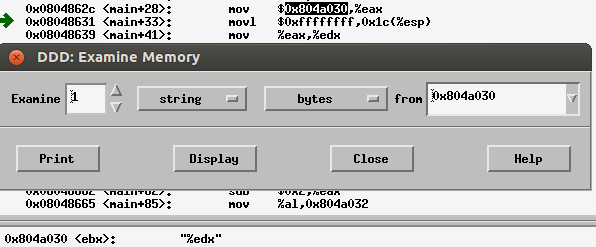
\includegraphics[scale=0.8]{capturas/figura1.png} 
		\caption{Primer indicio para averiguar la contraseña} 
		\label{fig:figura1}
	\end{figure}

	Como se aprecia, lo que se imprime es \textbf{\%edx} que es la contraseña inicial aún sin modificar. Esta cadena puede provocar cierto despiste por su nombre.
	\\
	
	Continuando la ejecución mediante \textbf{Nexti} de \textbf{Command Tool} se llega a un punto en el que la cadena $ " $sospechosa$ " $ anterior se va a modificar. En la Figura \ref{fig:figura2} aparecen tres lineas importantes. Basta con ver la primera para cerciorarse que la cadena se va a modificar. Mediante la herramienta anterior (memory) se comprueba la dirección
	\textbf{$ 0x804a032 $} y se ve que es \textbf{dx}. La siguiente instrucción lo qe hace es \textbf{restarle dos al valor 0x64} que se corresponde con la letra \textbf{d}.
	
	\begin{figure}[H] %con el [H] le obligamos a situar aquí la figura
		\centering
		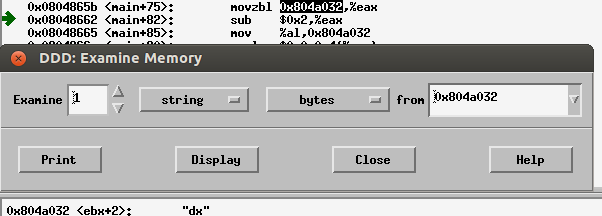
\includegraphics[scale=0.75]{capturas/figura2.png} 
		\caption{Segundo indicio para averiguar la contraseña} 
		\label{fig:figura2}
	\end{figure}

	Después de esas tres instrucciones se revelará un dato importante.
	Si se comprueba el valor de la misma dirección anterior (\textbf{$ 0x804a032 $}) ahora tendrá un nuevo valor: \textbf{bx}, tal y como muestra la Figura \ref{fig:figura3}
	
	\begin{figure}[H] %con el [H] le obligamos a situar aquí la figura
		\centering
		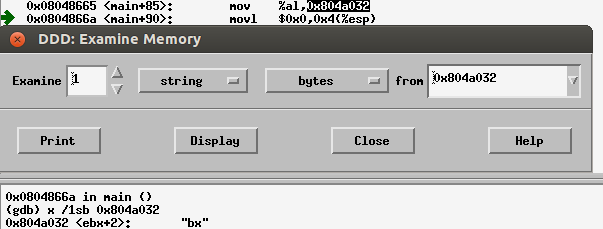
\includegraphics[scale=0.9]{capturas/figura3.png} 
		\caption{Tercer indicio para averiguar la contraseña} 
		\label{fig:figura3}
	\end{figure}
	
	Por último, comprobando el valor final que se queda en \%eax justo después de la llamada a \textbf{fgets} se obtiene la \textbf{contraseña}. En la Figura \ref{fig:figura4} puede verse la impresión del valor del registro y el obsequio de contraseña: \textbf{\%ebx}.
	
	\begin{figure}[H] %con el [H] le obligamos a situar aquí la figura
		\centering
		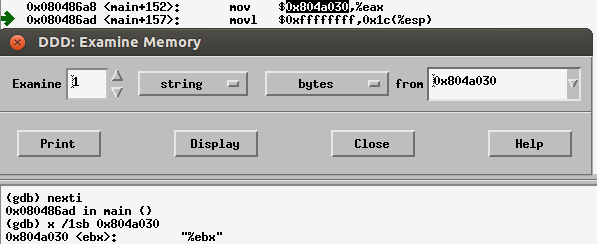
\includegraphics[scale=0.9]{capturas/figura4.png} 
		\caption{Obtención del valor de la contraseña} 
		\label{fig:figura4}
	\end{figure}

\newpage

\subsection{Código}
	Para obtener el código válido se va a proceder una estrategia parecida a la de la obtención de la contraseña.
	
	Recorriendo el código desde el principio con la herramienta \textbf{DDD}, poniendo un punto de ruptura en el comienzo del \textbf{main} se puede obtener el primer indicio para averiguar el código buscado. 
	\\
	
	Se llega a un punto en el que se realizan instrucciones $ " $sospechosas$ " $, como el de una multiplicación (instrucción señalada con la flecha en la Figura \ref{fig:figura5}). Como se ve en la Figura \ref{fig:figura5} el registro \textbf{\%eax}, con valor decimal 1892, se multiplica por el registro \textbf{\%edx}, con valor decimal 4.
	
	\begin{figure}[H] %con el [H] le obligamos a situar aquí la figura
		\centering
		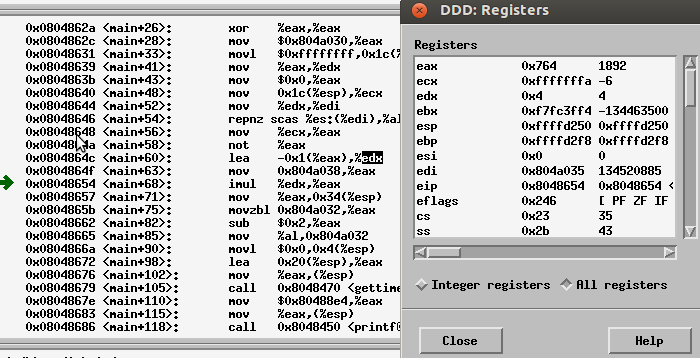
\includegraphics[scale=0.8]{capturas/figura5.png} 
		\caption{Primer indicio para averiguar la contraseña} 
		\label{fig:figura5}
	\end{figure}
	
	Una vez que se requiere que se introduzca el código, en este caso se introduce el \textbf{1111} para probar, se puede observar a continuación cómo es transformado su valor por el de \textbf{4444} antes de proceder a su comparación como se ve en la Figura \ref{fig:figura6}. 
	\\
	
	Es de aquí donde se puede afirmar que se realiza una multiplicación por 4 igual que se había visto anteriormente.
	
	\begin{figure}[H] %con el [H] le obligamos a situar aquí la figura
		\centering
		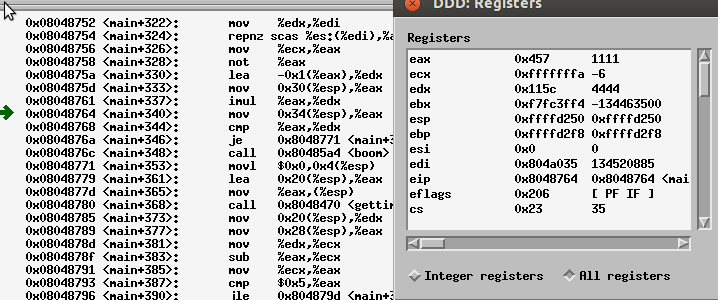
\includegraphics[scale=0.8]{capturas/figura6.png} 
		\caption{Primer indicio para averiguar la contraseña} 
		\label{fig:figura6}
	\end{figure}
	
	Por último aparece la parte crítica, en la que se corroborarán los resultados obtenidos hasta ahora o no. Dicha parte es la de la comparación, en la que se ve que se comparan los valores \textbf{7568} y \textbf{4444}, véase en la Figura \ref{fig:figura7}. El valor 7568 aparece como se vio anteriormente de la multiplicación de \textbf{1892 por 4} y 4444 es el código que se ha introducido por pantalla como prueba (1111) multiplicado también por cuatro.
	
	\begin{figure}[H] %con el [H] le obligamos a situar aquí la figura
		\centering
		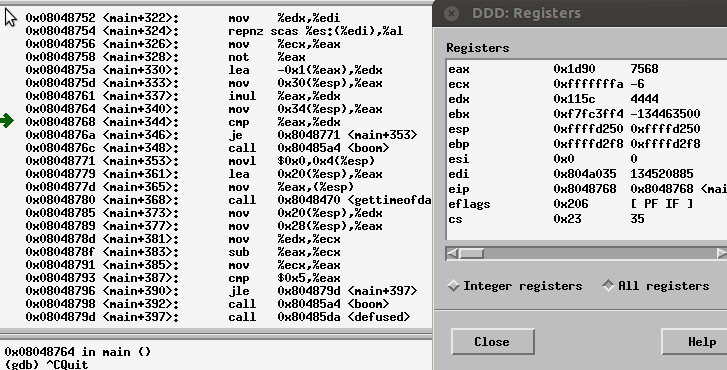
\includegraphics[scale=0.7]{capturas/figura7.png} 
		\caption{Primer indicio para averiguar la contraseña} 
		\label{fig:figura7}
	\end{figure}
	
	Gracias a la herramienta \textbf{Status} $ \rightarrow $ \textbf{Registers} de \textbf{DDD} ha sido posible seguir el transcurso de los registros y la modificación de sus valores en cada instrucción hasta conseguir el código final \textbf{1892}.
	
\newpage

\end{document}
